\chapter{Introduction}
\graphicspath{ {images/} }

\frenchspacing
For many years there has been no change in the basic structure of the power grids. Meeting the rising demand for electricity, measures to reduce equipment failures, reduction in the available fossil fuels, energy storage problems and the one way communication have posed a serious challenges on the electricity and transportation industries as described by  \cite{gungor2011smart}.  The energy grid has evolved from a centralized infrastructure to a complex system where every level of the distribution pipeline comprises of multiple smart devices which can connect to multiple power sources that can produce energy, as well as store it and exchange it with many other smart devices. The centralized nature of the power grid has been exchanged with the distributed systems which not only distribute the power but also exchange information which can improve efficiency, reliability and safety of the power grids. The existing grid is lack of communication capabilities, while a smart power grid infrastructure is full of enhanced sensing and advanced communication and computing abilities as illustrated in Figure \ref{fig:mesh}.

Power grids evolved with the integration of intelligent infrastructures and communication technology. These technologies not only made the power grids smart but also helped to achieve the goal of meeting the high demand power with the connection of energy produced from renewable resources and reducing the loss by employing smart technologies for detecting and minimizing power outages. These grids combine the  power and communication networks to connect homes, offices, and factories (consumers) to multiple distributed power providers (small-scale power generators) such as solar, wind, fuel cells, and facilities that store generated power. 

Smart grids will provide more electricity to meet rising demand, increase reliability and quality of power supplies, increase energy efficiency, integrate low carbon energy sources into power networks. Smart grids possess demand response capacity to help balance electrical consumption with supply, as well as the potential to integrate new technologies to enable energy storage devices and the large-scale use of electric vehicles \cite{abb}. 

Until the rise of Wi-Fi and mobile technology, power systems had very limited resources to detect the problem areas and resolve. Today, these capabilities are increasingly being employed by the power grids to give you update of the outages as soon as possible. The integration of smart devices to existing power distribution lines helps to monitor the state of the power grid, the operational conditions of the communication lines and respond for outages. Information are being communicated continuously determining the current operational conditions of the distribution lines, adding to the reliable transfer of power to the customers. 

Intelligent sensors deployed in smart grid network reduces the number of customers being impacted with the help of real-time outage response, which in turn restores the power to the affected areas in an alternative path. Addition to the automatic restoration, the affected area is isolated from the distribution network quickly which may have caused due to multiple reasons such as severe weather conditions, natural calamities and link breakages. 


\begin{figure}
\centerline{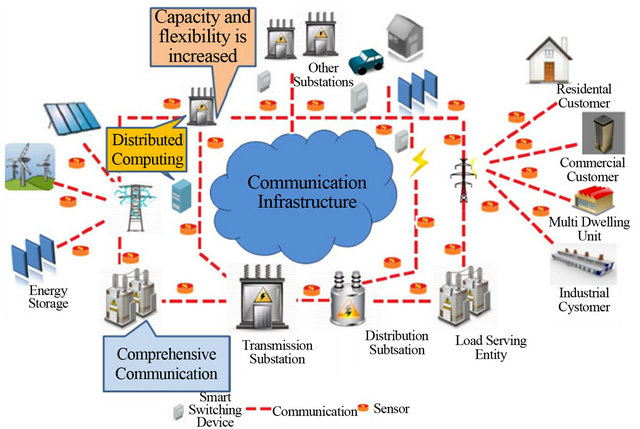
\includegraphics[totalheight=6cm]{smart_grid_infrastructure.png}}
    \caption{Smart grid architecture increases the capacity and flexibility of the net- work and provides advanced sensing and control through modern communica- tions technologies \cite{gungor2011smart}}
    \label{fig:mesh}
\end{figure}

\textbf{Data generated from smart grids: Delete this line after completing}

Apart from increased efficiency, self-restoration, operation automation, and renewable energy integration, the smart grids are potential sources of big data. The information technology support for the power transmission and distribution produces rapid amount of data. The sensors, the smart meters, the control units and the monitoring devices all add up to this huge volumes. Data are generated from various activities such as: power utilization habits of the users; phasor measurement data for situational awareness; energy consumption data measured by the widespread smart meters; energy market pricing and bidding data collected by advanced metering infrastructure; management, control and maintenance data of devices and equipment in the power generation, control data exchanged between transmission and distribution networks acquired by intelligent electronic devices \cite{lai2015big}. 

The grid is becoming more and more digital with the information recorded by the sensors and the smart meters deployed at the users' premises and along the grid and power stations. This data can be for example, consumption data from smart metering and electric vehicles, data telling about the conditions of the components in the grid \cite{aiello2014smart}. For achieving fine-grained monitoring and scheduling, information from the power grid needs to be collected within short intervals. 

\textbf{Energy saving using Smart grids}
\textbf{Effects of data, why are they collected : Delete this line after completing}

Collecting and managing, processing and analyzing electrical data reveals deeper insights that can help experts to improve the operation of power grid to achieve better performance. The technology to collect massive amounts of data is available today, but managing the data efficiently and extracting the most useful information out of it remains a challenge. Data obtained from the smart grids provides valuable information which helps for efficient grid operations. It is also closely related to the safety and reliability of the power system operation and management based on data-driven decision support. Using data from meters and sensors, an operator could be alerted that a transformer is having problems and help to make a decision from the information provided. For example, in the past when a transformer would fail, the lights would go out and the operator only knew about it when customers called. In future we would wish to have a sensor on the power line which sends an alert to the operator about that transformer. The operator recognizes where the outage is and dispatches a person to fix the problem. This gets the lights back on sooner and results in more satisfied customers \cite{Troiano}. 

With this technology, electrical utilities are equipped to deliver power more efficiently, improve operations, reduce emissions and management costs, and restore power faster. And operators are able to immediately identify outages, allowing for improved efficiency to manage responses. Smart grid data could also generate information on how individual customers respond to requests of consumption reduction. It is also possible to use real-time metering data to discover unaccounted consumption when energy is being diverted and stolen, reducing the cost of distribution operations. With smart meters, utilities can learn about the information of the number of units consumed by the user and the state of the grid. This information allows the power grids to deploy optimization techniques to find the optimal power generation, control mechanisms and transmission strategies for that state of grid.

 Construction and application of the smart grid have stimulated the accumulation of electric power grid operation data, production management data and electricity consumption data \cite{chen2016data}. The accumulated data contain redundant, missing and outlier data, resulting in serious issues of electric power data quality.  These electrical data can be used by data analytics researchers to obtain patterns and to make better decisions for electric utilization and control. They can make use of several techniques, including statistics, clustering algorithms, data mining, machine learning, signal processing, pattern recognition, optimisation and visualisation method to capture, curate, analyze and visualize the data. 

As there are advancement in technology, there are adverse effects as well. Over the last years power grids have been targeted with hazardous malware to steal their data and get access to their communication. Security is one feature which plays a very huge role in every communication entity. Since smart grids and the power generators exchange informations, intrusions, attacks and anomalies could occur because of malware activities. In order to accomplish these security goals we propose to use techniques which will be discussed in the later sections.

\begin{figure}
\centerline{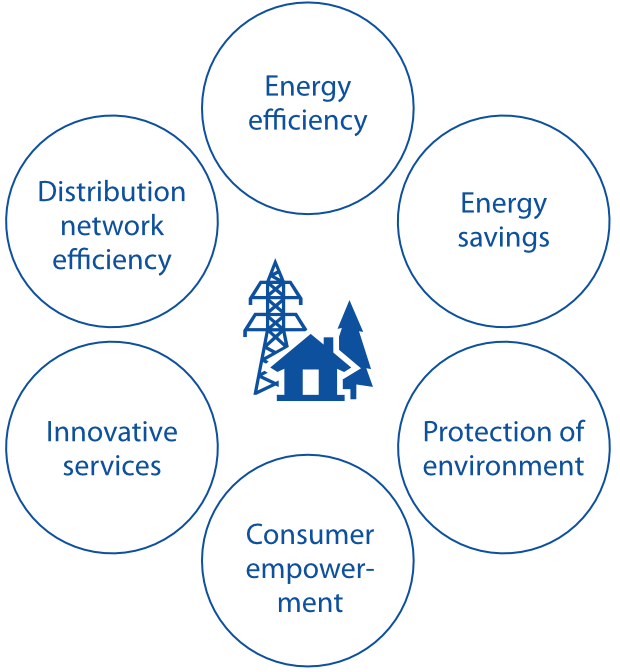
\includegraphics[totalheight=6cm]{SM_benefits.png}}
    \caption{Six ways the adoption of smart metering systems can benefit the electricity customer. 
    {Image src: http://www.foxconngfo.com/iot/foxconn/page-11.html}}
    \label{fig:SM_Benefits}
\end{figure}


\textbf{Our proposal for nullifying one of the effect: Delete this line after completing}
The massive amounts of measurement data that will be made available at distributed locations that can and must be leveraged to optimally operate the power grid.


\textbf{Added Newly: Should i write about how electricity is produced and transmitted, what are the tradeoffs to be considered when deploying the anomaly detection algorithms in the smart grids. }

In order to efficiently utilize the energy it requires one to study detailed knowledge of the energy usage patterns of the locations. For this we consider the energy usage patterns of the locations in order to identify irregularities of the transmitted energy. We do this by detection algorithms using the modern machine learning techniques. Apart  from  the  economic  benefit  brought along by the increased energy efficiency, there is also an urgent global need to reduce carbon emissions such as carbon dioxide,  which is closely tied up with the generation and hence consumption of electricity \cite{chan2012load}. Generally,  this  can  be  reduced  by  using  clean  (or cleaner) energy sources and the control of electricity consumption  or  demands  at  the  users’  side.
	The main aim of smart grids are to provide \begin{itemize}\item more efficient transmission of electricity. \item quicker restoration of electricity after power disturbances. \item reduced operations and management costs for utilities, and ultimately lower power costs for consumers. \item reduced peak demand, which will also help lower electricity rates. \item increased integration of large-scale renewable energy systems. \item better integration of customer-owner power generation systems, including renewable energy systems. \item improved security. \end{itemize}

Nevertheless, increased interconnection and integration also introduce vulnerabilities into the grid. Failure to address these problems will hinder the modernization of the existing power system. Through advanced sensing technologies and control methods, smart grids can capture and analyze data regarding power usage, delivery, and generation in near real-time. According to the analysis results, the smart grid may provide predictive information and corresponding recommendations to all stakeholders (e.g., utilities, suppliers, and consumers) regarding the optimization of their power utilization. It may also offer services like intelligent appliance control for energy efficiency and better integration of distributed energy resources (DERs) to reduce carbon emissions. Apparently, it is not a simple grid in the sense of our current power grid. It can be regarded as a “system of systems” that involves both information technology (IT) and electricity system operations and governance. Such a complex system undoubtedly presents many challenges, especially in cyber security and privacy aspects \cite{liu2012cyber}.

Smart grids should also consider the wide range of needs and power quality requirements. Power quality involves factors like voltage flicker, voltage volume, momentary interruptions, etc. Different consumers may have distinct power quality requirements (e.g., industrial vs. residential users). Optimizing the distribution of power by detecting the irregularities, outliers or anomalies will reduce power consumption. These timely detection of faults by using the proposed technologies will help in operating resiliently to disturbances, attacks and Natural disasters. Gann et al.  affirmed that cities become “smarter” when they exploit the increasing data and analytical techniques available, in order to improve energy effectiveness and efficiency through the integration of physical infrastructures and digital technologies \cite{gann2011physical}

\textbf{end}


The energy grid can now interact with the end user to control his energy consumption, by either direct control on some of his appliances (for example, the washing machine) or indirect control, by providing fine grain resolution on the cost of the energy at a given day and time, such that the final user tunes up his own schedule for the energy consumption. The grid can also promote cooperation among different prosumers (both producers and consumers of energy) to enable more efficient energy usage, particularly in what concerns consuming on the spot for renewable energies.

Discovering new information can be very beneficial to both power distribution grids and customers. Uncovering hidden energy usage patterns, identifying untapped energy efficiency opportunities, engaging customers for demand response programs by discovering high usage patterns, for instance, inefficient thermostat setpoints and charging their electric vehicles, can save a lot of energy and expenses of the customers \cite{ben7utilities}. 


Data is the fundamental currency of the smart grid. A clear understanding of how these data are generated, what it consists of, and the benefits it can be used to deliver is critical to realizing the fullest possible returns from smart grid investments. The benefit is to have enriched information of the performance of the system, its stability, and customer consumption. For this task, anomalies are of special interest, because they can be caused either by faulty equipment or potentially misconfigured devices consuming significantly more or less energy than required for proper operation.


Complex electric power system contains large amounts of real-time data. Data is accurate or not, which determines the safety and reliability of electric power system. Outlier data may affect the normal operation of electric power system and even threaten the security of entire system. Hence, in order to ensure the stable and safe operation of electric power system, it has important significances to extract and detect these outlier data from the original data. The significances of electricity consumption outlier data have two aspects on negative and positive influences.

The negative influences include the following aspects. Firstly, the presence of electricity consumption outlier data will reduce the accuracy of assessment. Then, the results of data mining cannot accurately reflect the characteristics of data. Finally, outlier data affect the judgement and decision of electric power system dispatcher \cite{huang2004enhancement}. It even threatens the safe operation of system. If outlier data cannot be correctly identified and effectively corrected, they will provide false prediction as a reference \cite{pham2014anomaly}. This affects the accuracy and reliability of prediction results. Furthermore, if outlier data are used as modeling data, it will interfere with the changing rules and influence the training accuracy. If outlier data are used as a predictor of test results, it can lead to erroneous judgement \cite{mao2005principle}.

Outlier detection of electricity consumption data is to find out the relatively sparse and isolated outlier data patterns which are hidden in massive data \cite{chen2016data}. In the early stage of data set preprocessing, we usually put outlier data as noise data. Although outlier detection finds the hidden data in the data set as the main purpose, outlier data mining is more valuable and meaningful than other types of mining [70]. Because one hundred thousand normal records are likely to cover only one rule, but ten outlier records are likely to cover ten different rules \cite{mao2005principle}, \cite{chen2016data}. Outlier detection of electricity consumption data may provide us more important information, so that we can find some real and unexpected knowledge, which can help us to understand the consumer behavior, capture the theft, find system vulnerabilities and failures and improve service quality \cite{pham2014anomaly} .

There is a growing interest in understanding how energy is spent in the commercial buildings. Furthermore, distributors of electricity want to know how to reduce the failure rate and detect anomalies which will serve the purpose of reliability and efficiency of the smart grid. In addition, they want to know how to visualize large volumes of energy data collected by power meters (sensors) in a building to find patterns, trends, and anomalies. In the end, our goal is to find how to automatically discover the anomaly, like unusual power consumption measurements highly differing from old observed patterns, and to reduce the energy cost of a building. For this task, anomalies are of special interest, because they can be caused either by faulty equipment or potentially misconfigured devices consuming significantly more or less energy than required for proper operation \cite{janetzko2014anomaly}.

\frenchspacing Vulnerabilities in power systems can cause a major disaster considering the large usage of electricity in today's world. A widespread loss of power even for few days, could make devices ranging from cellphones to ATMs to traffic lights, and even lives to halt, if heating, air conditioning and health care systems exhaust their backup utilities. But when dealing with infrastructure that may even be system-critical, the number of failures must be reduced to an absolute minimum. Early signs of failures should be visible in power usage patterns \cite{janetzko2014anomaly}. By detecting anomalies in the usage patterns of electricity, machine learning algorithms can help utilities take customer care a step further, helping them identify homes at greatest risk of switching providers, listen to their concerns, and offer solutions. Our motivation therefore, will be concentrated on finding the appropriate information from the collected smart grids data and to employ suitable discovery method on these data to detect vulnerabilities and/or anomalies in the data. 

\frenchspacing

\label{sec:Introduction}